\chapter{Ruta Óptima dentro el campus Universitario} % (fold)
\label{cha:ruta_optima}


Si se quiere ir de un punto a otro el mejor camino o el más óptimo siempre es aquel con la menor distancia entre los 2 puntos, pero como se puede definir que un camino es óptimo?, si se va en coche hay que tomar en cuenta la dirección de las calles, los cruces, etc. si se va a pie hay que ver las características del terreno, caminos cortados, distancias, etc.\\


Si se analiza el terreno que se va a cubrir con la aplicación (el campus de la UMSS ubicado entre las calles Oquendo, Sucre,  Belzu y M. U. Lopez), se tiene que el camino óptimo es siempre el más corto o de menor longitud, ya que el metodo de desplazamiento que se tomara en cuenta para moverse dentro del campus Univeristario sera \emph{a pie} y el terreno es plano.\\


La resolución de este problema es la se analizará en este capítulo.


  \section{Grafos} % (fold)
  \label{sec:teoria_grafos}

    El problema se lo podria definir como; Encontrar la ruta más corta de un punto a otro punto, en donde los puntos están interconectados por una red de caminos. El problema descrito se lo puede resolver/describir como un caso espec\'ifico de la teoría de grafos.


    \subsection{Definiciones} % (fold)
    \label{sub:grafos_definiciones}
      Primeramente es necesario aclarar\'ar alguno términos usados en la teoría de grafos.\\

      % El grafo que es la reprentacion

      % \begin{description}
      %   \item[Grafo] Un grafo G consiste en un conjunto  vértices V y un conjunto de aristas A, y se lo escribe como G(V,E).
      %   \item[Vertice]
      % \end{description}

      Un \textbf{grafo} $G$ consiste en un conjunto de vértices $V$ y un conjunto de aristas $A$, y se lo representa con $G(V,A)$.\\

      El \textbf{vértice} \emph{v} es adyacente a \emph{u}, o a un vecino de \emph{u}, si y sólo si $(u,v) \in A$. Por lo tanto, en un grafo no dirigido, dado una arista $(u,v)$, $v$ es adyacente de $u$, y simétricamente \emph{u} es adyacente de \emph{v}.
      Los vértices también son llamados nodos. \\

      Cada \textbf{arista} o arco es representada por un par de elementos $(u,v)$, donde los elementos $u,v \in V$, son los nodos que une la arista.
      En un grafo no dirigido el par de vértices que representan la arista no tiene orden, por lo tanto la arista $(u,v)$ y $(v,u)$ representa la misma arista. En cambio en un grafo dirigido la arista $(u,v)$ y $(v,u)$ representan dos diferentes aristas. También se puede anotar un tercer componente, llamado peso o costo, en ese caso estaríamos hablando de un \emph{grafo ponderado}.\\
      % Para fines prácticos, no  consideraremos las aristas de la forma (u,u)

      En un grafo no dirigido $G$, dos vértices $u$ y $v$ se dice que están conectados si hay un camino en $G$ de $u$ a $v$ (y como $G$ no es dirigido, también hay un camino de $v$ a $u$). Un grafo  se denomina completo si para todos los pares $u,v \in V$ existe una arista $(u,v) \in A$.\\

      Un camino en un grafo es una secuencia de nodos $v_{1}$, $v_{2}$, \ldots{}, $v_n$ tal que $(v_{1}, v_{2}), (v_{2}, v_{3}), \ldots{}, (v_{n-1}, v_n)$ son aristas.
    % \end{description}
    % subsection grafos_definiciones (end)
    \subsection{Representacion de un Grafo} % (fold)
    \label{sub:representacion_de_un_grafo}
      Existen diversas formas de representar un grafo sea dirigido o no-dirigido, pero entre las mas usadas están la matriz de adyacencias y la lista de adyacencias.
      \subsubsection{Matriz de adyacencias de un Grafo} % (fold)
      \label{ssub:matriz_de_adyacencias_de_un_grafo}
        Sea $G = (V,A)$ un grafo de \emph{n} vértices. La matriz de adyacencias $M$  para $G$ es una matriz $M_{nxn}$ de valores booleanos, donde $M(i,j)$ es verdad si y sólo si existe un arco desde el nodo \emph{i} al nodo \emph{j}.

        \begin{displaymath}
          M(i,j) = \left\{
          \begin{array}{ l l }
            1, & \textrm{si existe la arista } (i,j) \\
            0, & \textrm{en caso contrario}
          \end{array} \right.
        \end{displaymath}


        Las filas y las columnas de la matriz representan los nodos del grafo.
        Cuando el grafo no es dirigido la matriz de adyacencias es simétrica.
        % El cuadro \ref{tab:matriz} representa la matriz de adyacencias de la figura \ref{fig:grafo_ponderado} representa
        La matriz de adyacencias, que se puede observar en el cuadro \ref{tab:matriz}, es la  misma matriz de la relación $A$ de $V$ en $V$ porque indica cuales v\'ertices están relacionados (unidos por una arista).


        % \begin{tikzpicture}[->,>=stealth',shorten >=1pt,auto,node distance=3cm,
        %         main node/.style={circle,draw,font=\sffamily\Large\bfseries}]

        \begin{figure}[!ht]
          \begin{center}
            \caption{Grafo ponderado no-dirigido}
            \label{fig:grafo_ponderado}

            \begin{tikzpicture}[->,>=stealth',shorten >=1pt,auto,node distance=3cm,main node/.style={circle,draw,font=\sffamily\Large\bfseries}]

              \node[main node] (1) {a};
              \node[main node] (2) [below right  of=1] {b};
              \node[main node] (3) [above right of=2] {c};
              \node[main node] (4) [below left of=2] {d};
              \node[main node] (5) [right of=2] {e};
              % \node[main node] (6) [right of=5] {f};
              % \node[main node] (7) [above right of=6] {g};
              % \node[main node] (4) [below right of=1] {d};

              \path[every node/.style={font=\sffamily\small}]
                (1) edge node [auto] {3} (2)
                    edge node[left] {5} (4)
                (2) edge node[left] {8} (3)
                    edge node[right] {4} (4)
                    edge node[auto] {3} (5)
                (3) edge node[left] {7} (5)
                (4) edge node[below] {14} (5);

            \end{tikzpicture}

          \end{center}
        \end{figure}

        \begin{table}[!ht]
          \label{tab:matriz}
          \begin{center}
            \caption{Matriz de adyacencias del grafo de la figura  \ref{fig:grafo_ponderado}}
            \begin{displaymath}
              M(i,j) =
              \bordermatrix{ ~ & a & b & c & d & e \cr
                             a & 0 & 3 & 0 & 5 & 0 \cr
                             b & 3 & 0 & 8 & 4 & 3 \cr
                             c & 0 & 8 & 0 & 0 & 7 \cr
                             d & 5 & 4 & 0 & 0 & 14\cr
                             e & 0 & 3 & 7 & 14& 0  }
            \end{displaymath}
          \end{center}
        \end{table}


      % subsubsection matriz_de_adyacencias_de_un_grafo (end)

    % subsection representacion_de_un_grafo (end)
    \subsection{Ruta mas corta} % (fold)
    \label{sub:ruta_mas_corta}
      Dados los vértices $v_{i}$ y $v_{j}$ de un grafo $G = (V,A)$ se llama trayectoria mínima o camino minimo  de \(v_i\) a \(v_j\) al numero de aristas del camino de longitud mínima que va desde $v_i$ a $v_j$ y se representa por $d(v_i, v_j)$.

      Cuando en el grafo no exista un camino de $v_i$ a $v_j$ se dice que el camino minimo es $d(v_i, v_j) = \infty$ \\

      Para determinar el camino mínimo que va desde un único vértice a cualquier otro vértice se puede usar el algoritmo de Dijkstra.



      \subsubsection{Algoritmo de Dijkstra} % (fold)
      \label{sub:algoritmo_de_dijkstra}
      El algoritmo de  Dijkstra fue descrito en 1959 por \emph{Edsger Dijkstra}, y permite encontrar la trayectoria más corta entre dos nodos específicos, cuando los valores de los arcos son todos positivos\\

      El algoritmo asigna un etiqueta a cada nodo en el grafo. Esta etiqueta es la distancia que hay desde el nodo \emph{s} escogido como origen a lo largo de la trayectoria más corta encontrada, hasta el nodo que se está etiquetando.\\

      La etiqueta de cada nodo puede estar en 2 estados:

      \begin{itemize}
        \item[a.] Puede ser permanente: en este caso la distancia encontrada es a lo largo de la trayectoria, la más corta de todas las encontradas.
        \item[b.] Puede ser temporal: cuando hay incertidumbre de que la trayectoria encontrada sea la más corta de todas.
      \end{itemize}

      A medida que el método trabaja se cambian gradualmente las etiquetas temporales por etiquetas permanentes. Al comienzo se tiene un conjunto de nodos con etiquetas temporales y el objetivo es hacer que esas etiquetas disminuyan, encontrando trayectorias a esos nodos usando trayectorias a nodos etiquetados permanentemente. Cuando esto se ha logrado, se selecciona el nodo con la etiqueta temporal más pequeña y esta etiqueta se convierte en permanente. El proceso se repite hasta que al nodo terminal \emph{t} se le haya asignado una etiqueta permanente, pero esto puede ocurrir eventualmente, ya que cada vez que el algoritmo es usado, una de las etiquetas es omitida y así el número de nodos con etiquetas temporales decrece a cero. \cite{teoria_grafos} \\


      % subsection algoritmo_de_dijkstra (end)
    % subsection ruta_mas_corta (end)
  % section teoria_grafos (end)

  \section{Campus Universitario}
  \label{sec:ruta_corta_umss}

  En primer lugar fue necesario obtener un grafo ponderado no-dirigido que represente un mapa de los caminos que existen dentro del campus Universitario.\\

  Para obtener este mapa se procedió a caminar a través del campus de la UMSS con un GPS Garmin Nuvi 1300\footnote{El Garmin Nuvi 1300, es un dispositivo GPS básico pero cumple con el funcion de guardar información geográfica, los archivos generados tienen extensión gpx, el cual es básicamente un fichero XML estándar usado para compartir datos entre GPS's.}, se recorrieron los principales caminos que existen e interconectan las distintas facultades y oficinas dentro del campus universitario. Una vez realizado este recorrido, se procedió a extraer la información del dispositivo GPS, se utilizó el archivo \emph{current.gpx} para exportar la información  a un archivo \emph{shapefile}\footnote{Un shapefile es un archivo de formato sencillo y no topológico que se utiliza para almacenar la ubicación geométrica y la información de atributos de las entidades geográficas.\cite{what_is_shapefile} }, para esta tarea se utilizó QGis, con el cual se acabó editando las rutas recogidas por el GPS.\\


  Este paso fue necesario porque el mapa extraído del GPS es una línea única, pero para que nos sirva para el objetivo de buscar una ruta óptima, es necesario que esta línea sea dividida o separada en muchas líneas, las cuales son las aristas y los extremos de las líneas serán los nodos o vértices del grafo.\\

  Implementando el algoritmo de \emph{Dijkstra} en el grafo resultante es lo que nos permitir\'a encontrar la ruta más corta dentro del campus Universitario, al tener una gran cantidad de información resultante de la obtención de datos mediante un dispositivo GPS se hace imprescindible usar una base de datos que nos ayude con esta tarea, para lo cual se usó la base de datos PostgreSQL añadiendolo PostGIS y pgRouting, herramientas ampliamente utilizadas en el manejo de datos geo-espaciales.\\

   % el grafo representa el mapa de caminos  pueda ser usado en una base de datos  “ruteable”, esto significa que el mapa de una sola línea hay que separarlo o dividirlo en muchas líneas.\\


  Técnicamente esta línea única es representada como un \emph{POLYLINE} el cual consiste en una o más partes. Una parte es una secuencia conectada de dos o más puntos. Las partes pueden o no estar conectadas entre sí. Las partes pueden o no intersectarse entre sí, para transformar este POLYLINE necesitamos separar todas sus partes y convertirlas en objetos \emph{LINESTRING} únicos, y a este conjunto de LINESTRINGs es el que se va a usar en la base de datos como mapa de ``rutas''.\cite{esri_shapefile}\\

  \begin{figure}[H]
    \begin{center}
      \caption{Shapefile del campus Universitario.}
      \label{fig:shapefile_umss_v1}
      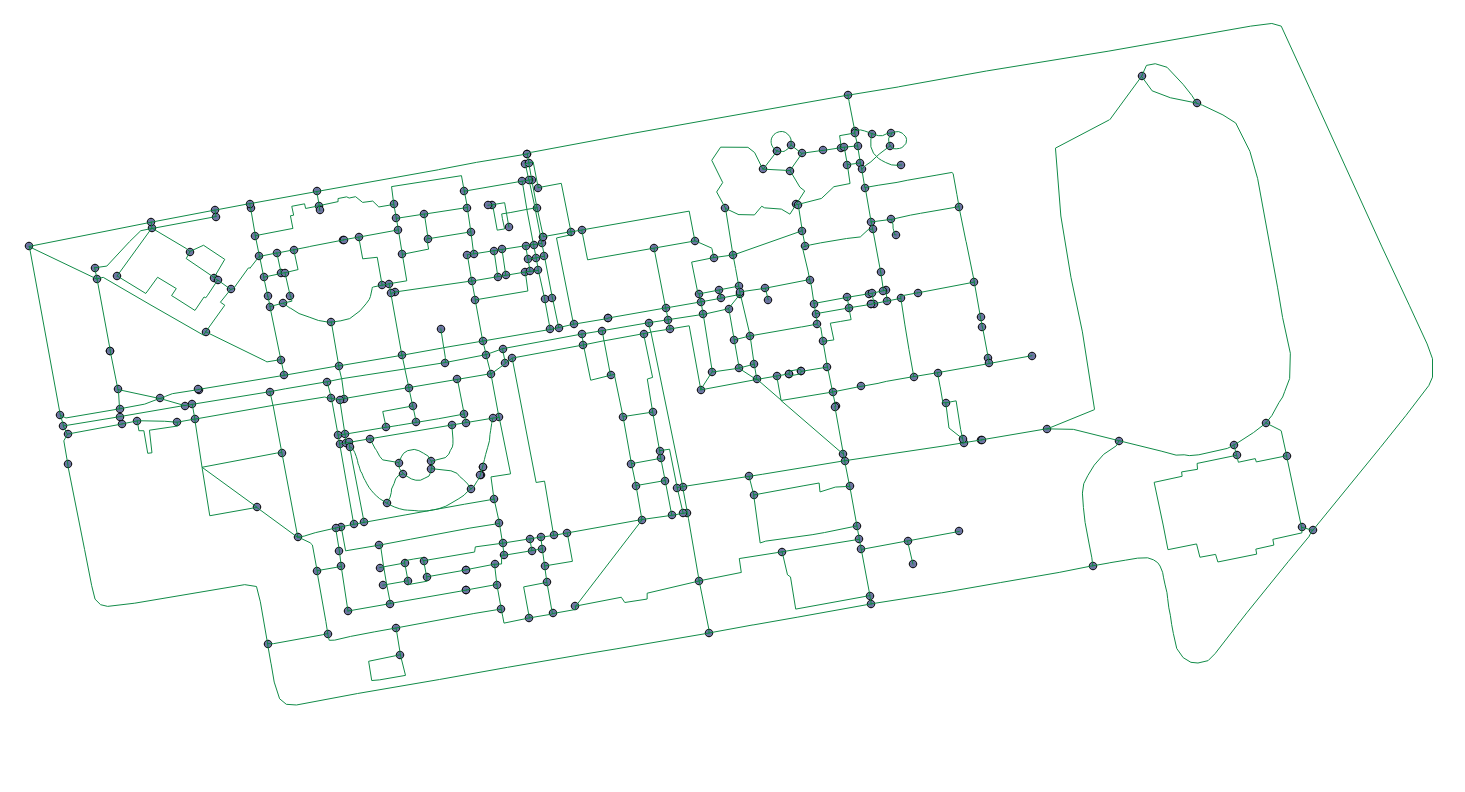
\includegraphics[width=1\textwidth]{shapefile_umss_v1}
      \caption*{Fuente: Elaboración propia}
    \end{center}
  \end{figure}

  En la figura \ref{fig:shapefile_umss_v1} se puede apreciar el shapefile resultante de la división del POLYLINE original, las líneas que conforman el mapa de las rutas del campus Universitario, donde cada línea es una arista y los puntos son los nodos del grafo no-dirigido, que será usado para la resolución del problema de la ruta más corta en el presente proyecto de grado.\\

  Para una mejor apreciación del grafo que consta de 1164 aristas y 1003 vértices, se lo puede ver en combinación o proyectada en un mapa de rutas del campus de la Universidad Mayor de San Simón ubicado entre las calles Oquendo, Sucre y  Belzu de la ciudad de Cochabamba - Bolivia, se puede referir a la siguiente figura \ref{fig:shapefile_umss_v2}.

  \begin{figure}[H]
    \begin{center}
      \caption{Campus Universitario de la UMSS ubicado en la calle Oquendo, Cochabamba-Bolivia.}
      \label{fig:shapefile_umss_v2}
      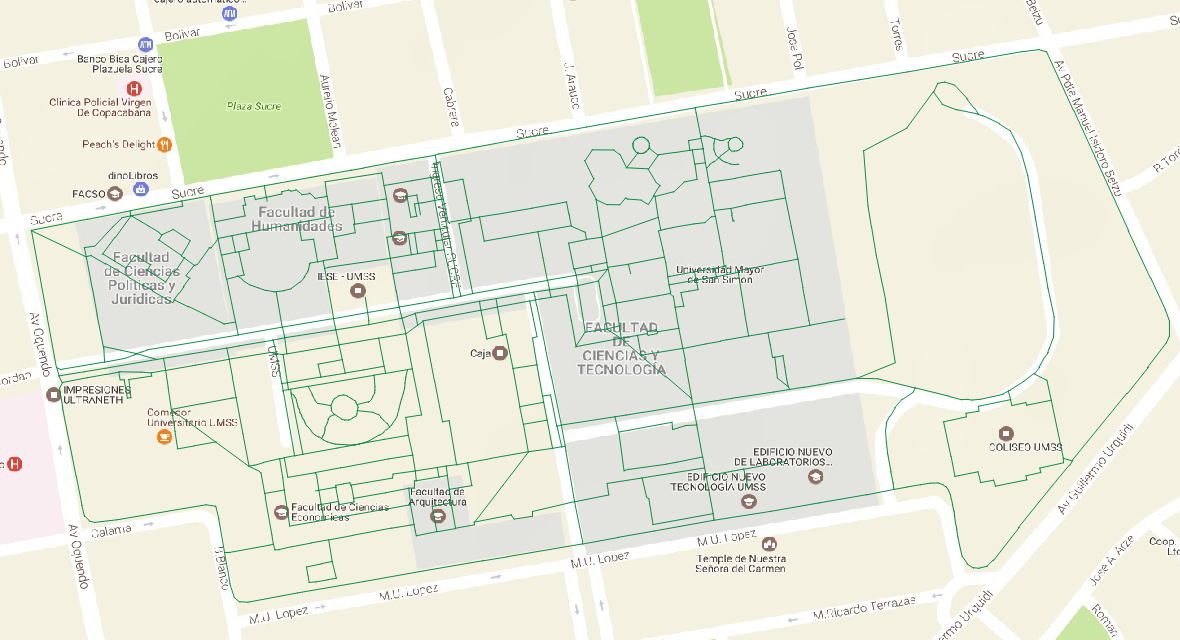
\includegraphics[width=1\textwidth]{shapefile_umss_v2}
      \caption*{Fuente: Elaboración propia}
    \end{center}
  \end{figure}


  \subsection{Facultad de Derecho}
  \label{sub:facultad_derecho}

  La facultad de Derecho cuenta con alrededor de 178 vértices y 88 aristas, está ubicada al nor-oeste del Campus Universitario, en la esquina de la calle Oquendo y Sucre, dentro del campus colinda con la facultad de Humanidades hacia el Nor-Este y hacia el Sur-Oeste está la facultad de Economía.

  \begin{figure}[H]
    \begin{center}
      \caption{Facultad de Derecho - UMSS}
      \label{fig:fac_derecho}
      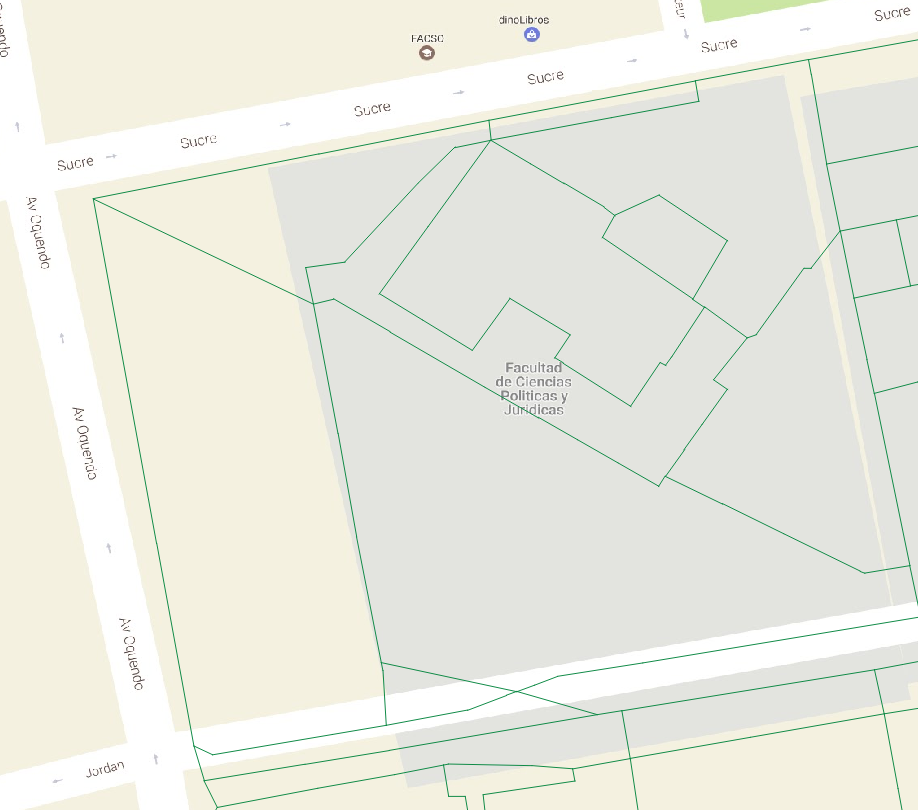
\includegraphics[width=1\textwidth]{fac_derecho}
      \caption*{Fuente: Elaboración propia}
    \end{center}
  \end{figure}

  En la figura \ref{fig:fac_derecho} se puede observar en la linea verde los caminos o rutas dentro de la facultad de derecho de la UMSS, proyectada sobre el mapa de Google Maps, para lograr esta representacion se utilizo QGIS ya que la informacion geografica de la ruta esta contenida en un archivo shapefile y el mapa se lo obtiene usando el API de Google Maps gracias al plugin de QGIS, \emph{QuickMapServices}\footnote{http://nextgis.com/blog/quickmapservices/}.


\subsection{Facultad de Economía}
\label{sub:facultad_economia}

La facultad de Economía está compuesta de XX aristas y XXX vértices, está ubicada en el sector Sur-Oeste del campus Universitario, colinda con las calles Oquendo y M. U. López, dentro del campus al Nor-Este se encuentra la facultad de Arquitectura y al Nor-Oeste la facultad de Derecho, tal como se puede apreciar en la figura \ref{fig:fac_economia}.

\begin{figure}[H]
  \begin{center}
    \caption{Facultad de Economia - UMSS}
    \label{fig:fac_economia}
    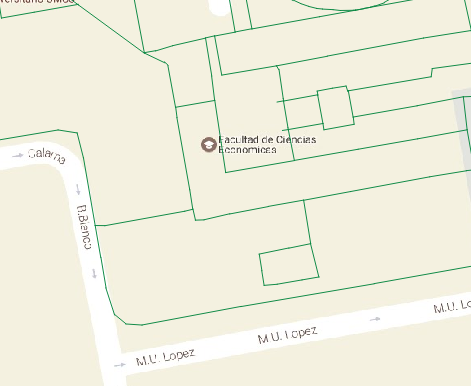
\includegraphics[width=1\textwidth]{fac_economia}
    \caption*{Fuente: Elaboración propia}
  \end{center}
\end{figure}



\subsection{Facultad de Humanidades}
\label{sub:facultad_humanidades}

La facultad de Humanidades está compuesta por XX aristas y XXX vértices, colinda con la calle Sucre hacia el Nor-Oeste, dentro del campus Universitario se encuentra la facultad de Tecnología hacia el Nor-Este, hacia el Sur-Oeste está la Facultad de Derecho y al Sur-Este se encuentra la Facultad de Arquitectura, en la figura \ref{fig:fac_humanidades} se puede apreciar la facultad de Humanidades dentro del campus Universitario sobrepuesto con el mapa de rutas identificado por la línea verde.

\begin{figure}[H]
  \begin{center}
    \caption{Facultad de Humanidades - UMSS}
    \label{fig:fac_humanidades}
    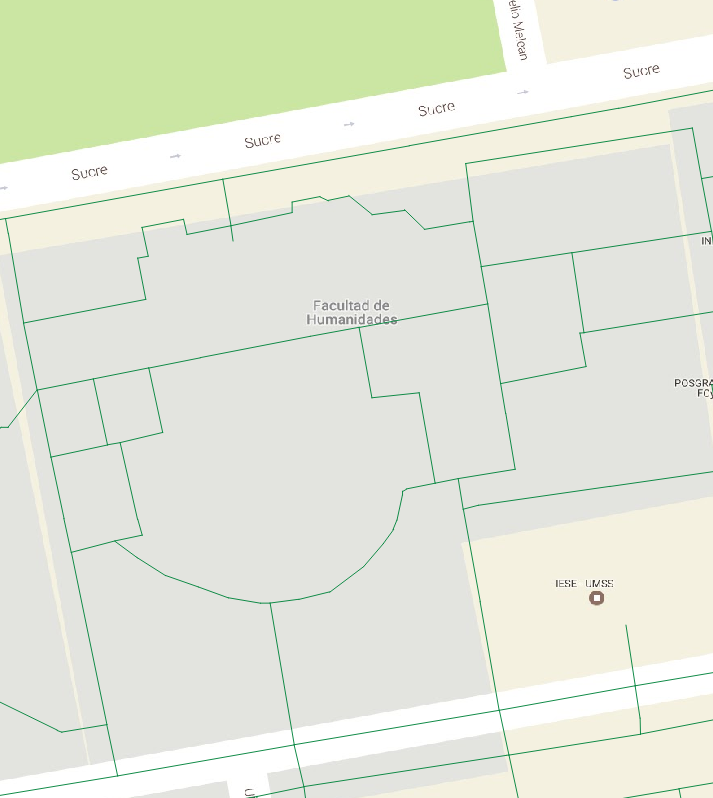
\includegraphics[width=1\textwidth]{fac_humanidades}
    \caption*{Fuente: Elaboración propia}
  \end{center}
\end{figure}


\subsection{Facultad de Tecnología}
\label{sub:facultad_tecnologia}

La facultad de Tecnología se encuentra en el extremo Nor-Este dentro del campus Universitario y cuenta con XX aristas y XXX vértices, la facultad de tecnología colinda hacia el Nor-Oeste con la calle Sucre, y hacia el Este con la calle Belzu, dentro del campus Universitario colinda con las facultades de Arquitectura y Humanidades que se encuentran hacia el Sur-Este y Sur-Oeste correspondientemente, en la siguiente figura \ref{fig:fac_tecno} se puede apreciar el mapa de rutas de la facultad de Tecnología.

\begin{figure}[H]
  \begin{center}
    \caption{Facultad de Tecnologia - UMSS}
    \label{fig:fac_tecno}
    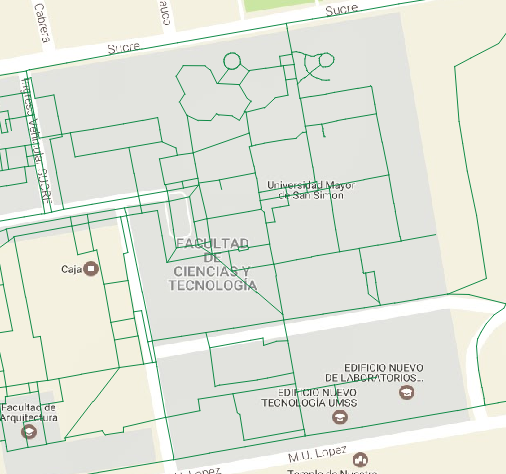
\includegraphics[width=1\textwidth]{fac_tecno}
    \caption*{Fuente: Elaboración propia}
  \end{center}
\end{figure}

\subsection{Facultad de Arquitectura}
\label{sub:facultad_arquitectura}

El grafo correspondiente a la facultad de Arquitectura cuenta con XX aristas y XXX vértices, la facultad colinda con la calle M. U. Lopez, dentro de los predios del campus Universitario se halla entre las facultades de Economía hacia el Sur-Este y con la facultad de Tecnología hacia el Nor-Oeste, el grafo se puede apreciar en la siguiente figura \ref{fig:fac_arqui}.

\begin{figure}[H]
  \begin{center}
    \caption{Facultad de Arquitectura - UMSS}
    \label{fig:fac_arqui}
    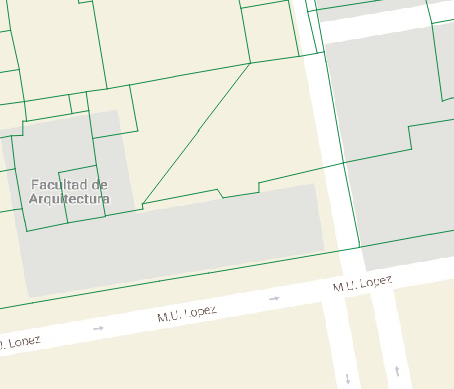
\includegraphics[width=1\textwidth]{fac_arqui}
    \caption*{Fuente: Elaboración propia}
  \end{center}
\end{figure}


  \section{Conclusi\'on} % (fold)
  \label{sec:ruta_conclusion}

    Existen numerosas soluciones para encontrar la ruta óptima, donde se toman en cuenta diferentes variables y heurísticas, en el que  cada algoritmo presenta ventajas respecto a las demás.
    La teoría de grafos  es un tema extenso y para fines prácticos
    solo se explicó el algoritmo de Dijkstra por ser el que se esta usando en la aplicación desarrollada.\\

    El algoritmo de Dijkstra puede ser una de las soluciones más sencillas y que requiere muchos más cálculos que las demás pero el grafo implementado al no ser extenso, por extenso se podria entender un grafo con millones de aristas y vertices como se puede dar en el caso de una Ciudad o un Pais, pero en el presente caso al ser los predios de campus Universitario no existe una razón de gran peso para implementar otra solución más eficiente en el manejo de recursos.\\

    El problema de la ruta más corta es ampliamente usado por las empresas de transporte, correos, etc., que necesitan mejorar la eficiencia del trayecto y a la vez reducir el consumo de combustible, dentro del campus universitario, reducir el tiempo en el cual encontramos un aula o una oficina mejoraría en gran medida la presentación de la Universidad hacia gente externa que necesitan hacer uso o encontrar algún lugar en especifico ya que lamentablemente esta información actualmente sólo te la pueden ofrecer las personas que conocen el lugar de antemano y aun en esos casos existe la posibilidad de no encontrar el lugar que se está buscando.\\




  % section ruta_conclusion (end)
% chapter ruta_optima (end)


  % Algoritmos de busqueda de caminos - ruta corta

  % Como determino que tipo de grafo tengo


  % % \section{La Red} % (fold)
  % % \label{sec:la_red}

  % % % section la_red (end)

  % \section{Algoritmo} % (fold)
  % \label{sec:algoritmo}

  % % section algoritmo (end)

  % \section{Algoritmo de Dijkstra} % (fold)
  % \label{sec:algoritmo_de_dijkstra}

  % % section algoritmo_de_dijkstra (end)

  % % Por lo tanto se implementó un grafo no dirigido (sin dirección), el cual se analizará en este capítulo.


  % Un problema de este tipo es represetable como un proble de teoria de grafos.


  % Cuando se tiene que encontrar un camino o ruta optima entre 2 puntos, se tienen que tomar en cuenta varios puntos


  % El problema de encontrar una ruta optima entre 2 puntos se lo puede resolver/representar como problema de grafos


  % Caminos mínimos en grafos

  % Solución voraz: Algoritmo de Dijkstra

  % para grafos dirigidos (la extensión a no dirigidos es inmediata)
  % genera uno a uno los caminos de un nodo v al resto por orden creciente de longitud
  % usa un conjunto de vértices donde, a cada paso, se guardan los nodos para los que ya se sabe el camino mínimo
  % devuelve un vector indexado por vértices: en cada posición w se guarda el coste del camino mínimo que conecta v con w
  % cada vez que se incorpora un nodo a la solución se comprueba si los caminos todavía no definitivos se pueden acortar pasando por él
  % se supone que el camino mínimo de un nodo a sí mismo tiene coste nulo
  % un valor en la posición w del vector indica que no hay ningún camino desde v a w
  % E.W. Dijkstra:
  % “A note on two problems in connexion with graphs”,
  % Numerical Mathematica, 1, pp. 269-271, 1959.
